\documentclass{article}
%\documentclass{exam}
\usepackage[italian]{babel}
\usepackage[T1]{fontenc}
\usepackage{graphicx}
\usepackage[utf8x]{inputenc}
\usepackage{amsmath}
\usepackage{amsthm}
\usepackage{hyperref}
\usepackage{subcaption}
\date{Dicembre 2018}
\author{Francesco Sacco}
\title{Oscillatore di Wien}

\begin{document}
\maketitle
\paragraph{1)}
	Per il primo punto ho usato un segnale in ingresso $V_s$ con un ampiezza picco picco di $260\pm11 mV$, e ho fatto delle misurazioni con dei segnali con frequenza compresa tra i $500$Hz e $3$kHz. I valori delle misure e i grafici sono riportati qui sotto\newline
	\begin{center}
		\begin{tabular}{cccc}
\hline
	$f$[kHz] & $V_A$[mV] & $V_A/V_{in}[dB]$ & fase [gradi]\\ 
\hline
	$0.4495\pm0.00001$ & $(1.25\pm0.05)\times 10^{2}$ & $-6.4\pm0.5$ & $43.4\pm0.9$ \\
	$0.6811\pm0.00001$ & $(1.55\pm0.07)\times 10^{2}$ & $-4.5\pm0.5$ & $29.4\pm0.6$ \\
	$1.0047\pm0.0001$ & $(1.72\pm0.09)\times 10^{2}$ & $-3.6\pm0.6$ & $15.9\pm0.3$ \\
	$1.2169\pm0.0001$ & $(1.78\pm0.09)\times 10^{2}$ & $-3.3\pm0.6$ & $9.0\pm0.2$ \\
	$1.5983\pm0.0001$ & $(1.82\pm0.09)\times 10^{2}$ & $-3.1\pm0.6$ & $0\pm 8.0\times 10^{-2}$ \\
	$2.17434\pm0.00001$ & $(1.74\pm0.09)\times 10^{2}$ & $-3.5\pm0.6$ & $-11.6\pm0.2$ \\
	$2.89413\pm0.00001$ & $(1.66\pm0.08)\times 10^{2}$ & $-3.9\pm0.6$ & $-24.2\pm0.5$ \\
\hline
\end{tabular}

	\end{center}
	\begin{figure}[htb]
	    \begin{minipage}[t]{.5\linewidth}
	        \centering
	        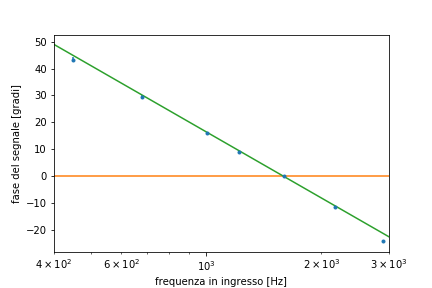
\includegraphics[width=\linewidth]{figure/1.png}
	        \subcaption{sfasamento del segnale in funzione della frequenza in ingresso}
			\label{fig:1}
	    \end{minipage}
	    \begin{minipage}[t]{.5\linewidth}
	        \centering
	        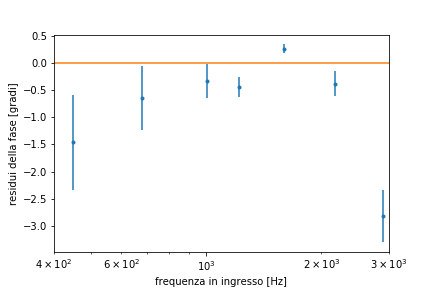
\includegraphics[width=\linewidth]{figure/1res.png}
	        \subcaption{Residui dello sfasamento}
			\label{fig:1res}
	    \end{minipage}
	    \caption{sfasamento}
	\end{figure}
	\begin{figure}[h!]
		\centering
		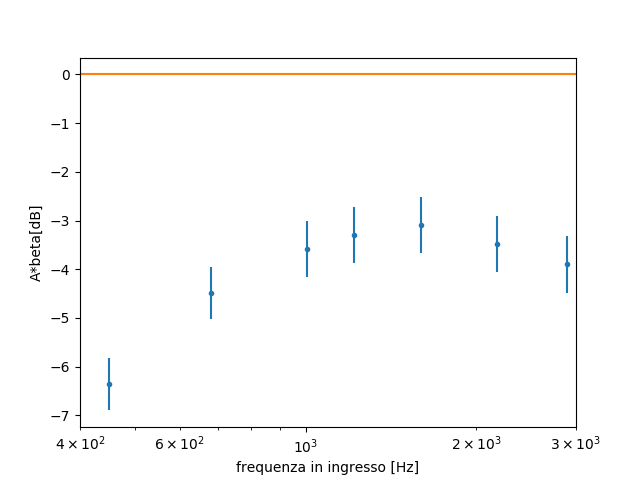
\includegraphics[width=\linewidth]{figure/2.png}
		\caption{Attenuazione del segnale in funzione della frequenza in infresso}
		\label{fig:2}
	\end{figure}
	dalla figura \ref{fig:1} si evince chiaramente che lo sfasamento diminuisce al'aumentare della frequenza e si ha uno zero alla frequenza di taglio $f_t=1/2\pi\sqrt{R_1R_2C_1C_2}$, i valori delle componenti indicate nel circuito in figura \ref{fig:circ1} sono disponibili nella lista qui sotto
	\begin{itemize}
		\item $R_1=9.99\pm0.08k\Omega$
		\item $R_2=9.91\pm0.08k\Omega$
		\item $R_3=9.93\pm0.08k\Omega$
		\item $R_4=9.88\pm0.08k\Omega$
		\item $R_5=9.97\pm0.08k\Omega$
		\item $C_1=11.1\pm0.4nF$
		\item $C_2=9.8\pm 0.4nF$
	\end{itemize}
	Ne consegue che $f_t=1.5\pm0.4 k$Hz\footnote{L'errore risulta grande perchè quando ho propagato $R_1R_2C_1C_2$ sull'inverso della radice, essendo la derivata intorno allo zero molto alta l'errore è esploso. Infatti\newline $R_1R_2C_1C_2=(1.07\pm 0.06)\times 10^{-8}$}. Essendo in un regime con frequenze vicine a quella di taglio mi sono permesso di fare un fit lineare per vedere nel grafico dei residui gli errori (fig \ref{fig:1res})\newline
	\begin{figure}[htb]
	    \begin{minipage}[t]{.5\linewidth}
	        \centering
			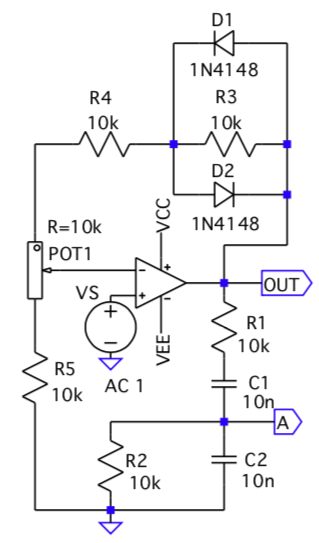
\includegraphics[width=\linewidth]{figure/circ1.png}
			\subcaption{Circuito senza feedback}
			\label{fig:circ1}
	    \end{minipage}
	    \begin{minipage}[t]{.5\linewidth}
	        \centering
			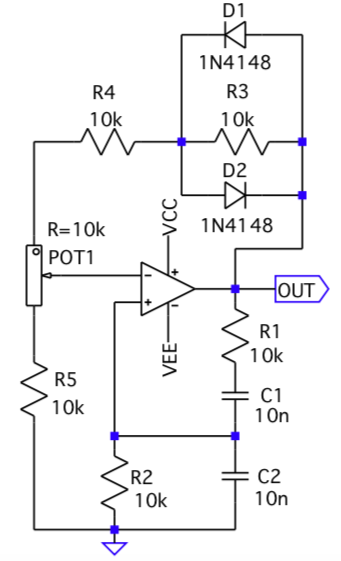
\includegraphics[width=\linewidth]{figure/circ2.png}
			\subcaption{Circuito con feedback}
			\label{fig:circ2}
	    \end{minipage}
	\end{figure}
	Per quanto riguarda l'attenuazione si nota dall'immagine \ref{fig:2} un massimo nella frequenza di taglio, mentre le altre frequenze vengono attenuate di più.\newline
	Il valore teorico dell'attenuazione è $|A\times\beta(f)|$ dove $A$ è l'attenuazione del partitore di tenzione messo a feedback, mentre $\beta(f)=\frac{iff_t}{f_t^2+3ff_t-f^2}$ è l'attenuazione del partitore di tenzione generalizzato composto dalle resistenze e capacità.\newline

	Per verificare la dipendenza del guadagno dal segnale in ingresso $V_S$ ho fatto un pò di misure che sono mostrate qua sotto, in particolare il guadagno diminuisce all'aumentare di $V_S$.\newline
	\begin{minipage}{.4\linewidth}
        \centering
        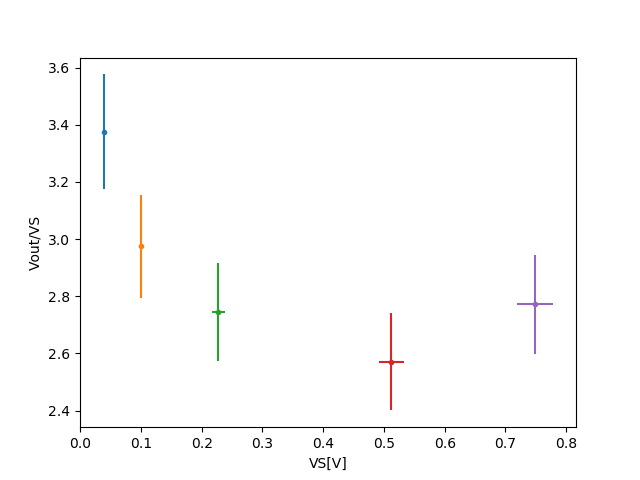
\includegraphics[width=\linewidth]{figure/1b.png}
    \end{minipage}
    \begin{minipage}{.5\linewidth}
        \begin{tabular}{ccc}
\hline
	Nome & Voltaggi misurati $[V]$ & Voltaggi datasheet $[V]$\\ 
\hline
	VOH & $4.1\pm0.2$ & 3.4 \\
	VOL & $0.134\pm0.006$ & 0.2 \\
	VIH & $1.16\pm0.05$ & >2 \\
	VIL & $0.74\pm0.03$ & <0.8 \\
\hline
\end{tabular}

        \label{tab:124}
    \end{minipage}
\paragraph{2)}
	girando il potenziometro il segnale aumenta o diminuisce di ampiezza, ma ha sempre una frequenza pari a quella di taglio, quando l'amplificazione $A$ scende sotto $1/\beta$ il circuito smorza ogni frequenza, rendendo nullo il segnale.
\paragraph{3)}
	La frequenza varia in modo insignificante al variare della posizione del potenziometro, infatti la frequenza massima e quella minima misurata al variare della posizione del potenziomentro sono rispettivamente $f_{max}\approx1.549 kHz$ e $f_{min}\approx1.541 kHz$.\newline
	Come detto prima l'ampiezza è il parametro che varia di più al variare dell'oscillazione, purtoppo mi sono scordato a misurare l'ampiezza massima e quella minima
\paragraph{4)}
	Misurando con l'oscilloscopio i voltaggi si ottiene che $V_{A}=242\pm1mV$ e $V_{out}=716\pm3mV$, facendo il rapporto si ottiene $V_{out}/V_{A}=2.9\pm0.2$, che è in linea con la teoria
\paragraph{5)}
	Levando i due diodi il segnale aumenta il voltaggio in uscita fino a $26.5\pm1.1 V$, e si ha un leggero clipping del segnale, come in figura \ref{fig:clipping1}.\newline
	All'allontanarsi dalla posizione dell'innesco dell'oscillazione la forma d'onda di distorce, la frequenza diminuisce, ma il voltaggio di clipping rimane costante (figura \ref{fig:clipping2}).
	\begin{figure}[htb]
	    \begin{minipage}[t]{.5\linewidth}
	        \centering
			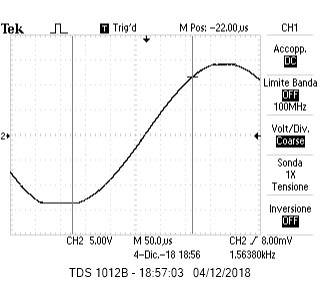
\includegraphics[width=\linewidth]{figure/clipping1.png}
			\subcaption{Clipping del circuito quando la posizione del potenziometro è vicino all'innesco dell'oscillazione}
			\label{fig:clipping1}
	    \end{minipage}
	    \begin{minipage}[t]{.5\linewidth}
	        \centering
			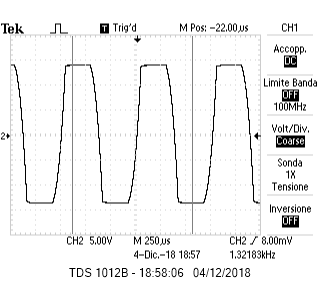
\includegraphics[width=\linewidth]{figure/clipping2.png}
			\subcaption{Clipping del circuito quando la posizione del potenziometro è lontano dall'innesco dell'oscillazione}
			\label{fig:clipping2}
	    \end{minipage}
	\end{figure}
	Viceversa se quando si ci trova alla posizione d'innesco si gira il potenziometro nella direzione opposta a prima il segnale scopare.
\end{document}